In this chapter, we discuss background information on the control-flow attacks and possible remedies against them. We also provide background information on specifics of ELF binaries in the context of position-independent code. Finally, we touch upon the Spectre vulnerability and how it affected the design of our re-randomization technique.


\section{Return-Oriented Programming (ROP)}
\label{sec:bg_rop}
\subsection{Stack Smashing Attack}

A \textit{buffer overflow} occurs when the data being written to a buffer overflows its boundaries and overwrites adjacent memory locations. A buffer overflow bug can be exploited by an attacker to manipulate the program to their advantage in what is known as a \textit{buffer overflow attack}.
A typical example of code vulnerable to buffer overflow attacks is described in Listing~\ref{lst:buffer_overflow}. The program takes a string from the command line and copies it to a local variable |buffer| in the function |foo|. A C library function |strcpy|, which is used for copying strings, just blindly copies the source into destination until a null terminator is reached.

\lstset{language=C}
\begin{lstlisting}[frame=single, caption={Buffer Overflow Example Code},label={lst:buffer_overflow}]
#include <string.h>

void foo(char *str){
    char b[8];
    strcpy(b, str);
}

int main(int argc, char **argv){
   foo(argv[1]);
   return 0;
}
\end{lstlisting}

The code in Listing~\ref{lst:buffer_overflow} works as expected for input strings of 7 characters or less (1 byte is used to store the null terminator to indicate the end of the string). A scenario when the string |HELLO| is passed to the function is illustrated in Figure~\ref{fig:stack_overflow_1}. The string including the null terminator is copied to the memory location |b[0]| to |b[5]|. The string passed is written within the confines of the buffer and the program behaves as intended.

\begin{figure}[ht!]
\centering
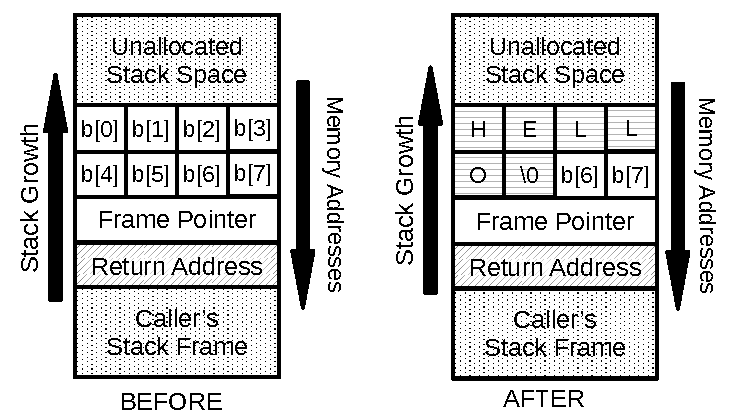
\includegraphics[width=0.7\columnwidth]{pictures/stack_overflow_1.pdf}
\caption{Snapshot of the stack before and after strcpy is called with safe input}
\label{fig:stack_overflow_1}
\end{figure}

When the function |foo| is called with an argument larger than 7 characters, the |strcpy| function overwrites the local variables defined in |foo|, the frame pointer and, most importantly, also the return address. When the |foo| function returns, the now compromised return address is loaded into the program counter and the control flow jumps to a new location instead of back to |main|. This situation is shown in Figure~\ref{fig:stack_overflow_2}. Here the command line input is ``AAAAAAAAAAAA\x02\x46\xA0\x88'', where ``AAAAAAAAAAAA'' is the code the attacker wants to execute and ``\x02\x46\xA0\x88'' is the little endian representation of the address of the local variable |b[8]| (the location in memory that contains the injected code). Note that in an actual attack, the attacker will likely put shellcode in the buffer and this way when the function |foo| returns, the shellcode would be executed, a shell would be launched and the attacker would have to ability to launch any arbitrary program.

\begin{figure}[ht!]
\centering
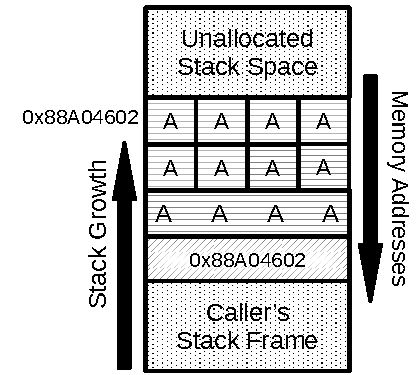
\includegraphics[width=0.35\columnwidth]{pictures/stack_overflow_2.pdf}
\caption{Snapshot of the stack after strcpy is called with unsafe input}
\label{fig:stack_overflow_2}
\end{figure}

Over the years various schemes have been developed to prevent this kind of attack. The most popular technique is data execution prevention. This technique uses a feature in modern CPUs called the Write-XOR-Execute ($W\oplus X$), also known as the NX (No-Execute) bit in x86-64 ~\cite{NXLINUX}. This feature allows memory regions to be marked as non-executable, i.e., any attempt to execute code from these regions would be prevented and an exception would be generated. The idea here is to keep all regions in memory either executable or writable but never both. Since modern operating systems mark all data pages as NX~\cite{UBUNTUNX}, this form of attack is no longer possible.

\subsection{Return-to-libc Attack}
After code injection attacks were effectively foiled by data execution prevention, a new genre of attacks known as code reuse attacks came into existence. One such attack is a return-to-libc attack. In this attack, the malicious entity does not inject code into the stack, but instead, an attacker pivots the stack to a carefully crafted call stack in memory. This way the attacker can chain the executions of a set of |libc| functions and orchestrate desired malicious behavior~\cite{nergal}. This attack goes around NX protection because the code is never executed from the stack itself but from the already existing libc code.

\subsection{Return-Oriented Programming}
Return oriented programming is a more generalized variant of the return-to-libc attack. In this technique, an attacker diverts the program control flow, but instead of jumping to a library function, a carefully chosen machine instruction already present in the code is executed. These machine instructions are called ``gadgets''. Each gadget typically ends with a return instruction. After a gadget is executed, a return address is popped from the stack into the program counter; this address is the address of the next gadget. Thus by crafting a call stack, the attacker is able to chain arbitrary machine instructions together to achieve the desired behavior. 

Figure~\ref{fig:rop_ex} illustrates how an ROP attack works. In the example, the attacker has injected three return addresses onto the stack, each pointed to a code gadget. When the original function returns, the |return address 1| is popped from the stack and the program jumps to gadget 1. When gadget 1 returns, the program jumps to the next injected return address (|return address 2|). One by one all the gadgets are executed causing the CPU to perform arbitrary actions.

\begin{figure}[ht!]
\centering
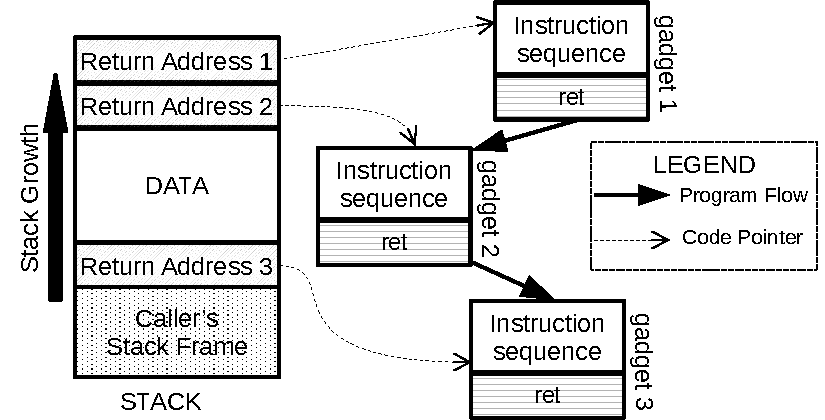
\includegraphics[width=0.65\columnwidth]{pictures/rop-min.pdf}
\caption{ROP illustration}
\label{fig:rop_ex}
\end{figure}

ROP's fundamental premise is that, given a large enough set of already loaded instructions, one can piece together a sequence of instructions that is  valid on a given ISA and accomplishes the desired malicious goal. The high density of ISAs, in particular ISAs such as x86-64, make the task of finding such a sequence of bytes or instructions easier. 

ROP is Turing-complete~\cite{Buchanan:2008:GIG:1455770.1455776}, meaning, given a sufficiently large program binary, any desired functionality can be emulated by chaining a sufficient number of gadgets. Several tools have recently been developed that can automatically create ROP payloads from program
binaries~\cite{ROPCOMPILER} -- e.g., the ROPgadget tool~\cite{ropgadget} can create an attack payload that spawns a shell that can accept arbitrary commands from an attacker.


\section{Supporting ASLR}
\label{sec:bg:aslr}
ASLR (address space layout randomization) is a widely adopted technique used to prevent exploitation of memory corrupting vulnerabilities such as stack smashing attacks. Before the advent of ASLR, operating systems would simply load an executable at a fixed address in virtual memory. With ASLR enabled, an executable or a shared library could be loaded at any random address.
At compilation time, the linker is unaware of where the code/data might be loaded, this means that the code can not directly reference other code or data in memory. In this section we discuss the two main approaches to solve this problem in Linux.

\subsubsection*{Load-Time Relocation}
A relatively straight forward way of solving this problem is to perform a load-time relocation. In load-time relocation, all the code/data references in a program are patched by the |dynamic loader| when the load address of the program is determined.

Load-time relocation has two fundamental problems.
First, it takes time to perform relocations. A complex software may reference a large number of libraries, patching each of these libraries at start-up could cause significant delays in program launch time.
Secondly, load-time relocation inhibits sharing of library code. %especially in x64 architectures. Thanks to variable/function addressing in x64 unless each program loads the library at the exact same virtual address, sharing of library code is not possible.
Loading the library at the same address is a security concern and defeats the purpose of ASLR. Therefore, the library would have to be loaded again in memory for each process that needs it. Since saving RAM is one of the most important points of having a library, using this approach is out of the question.

\subsubsection*{Position-Independent Code (PIC)}
\label{sec:bg:pic}
PIC relies on two key ideas, i.e. relative addressing and indirection. Firstly even though the program when loaded at a random address would not be able directly reference code/data, the relative offsets between code and data sections remain the same. The linker is aware of all the sections and their respective sizes at compile time and can generate code that can reference parts of the program using this already known offset. Such code uses the ``RIP-relative'' addressing mode~\cite{INTEL,AMD} in x86-64, where 32-bit offsets are added to the instruction pointer, effectively allowing the program to execute anywhere in the 64-bit virtual address space.

Most programs use dynamically linked shared libraries. Using the aforementioned RIP-relative addressing is not a suitable approach to reference a shared library because the position of the shared library relative to a program load location is arbitrary and unknown. Hence PIC adds an additional level of indirection to all library references (for both data and function calls). This indirection is implemented using Global Offset Table (GOT), discussed in Section~\ref{sec:background_got}, and Procedure Linkage Table (PLT), discussed in Section~\ref{sec:background_plt}.

The PIC model first advocated in~\cite{LIBCRET} provides support for ASLR without the limitations of Load-Time Relocation and is steadily gaining increasing popularity in Linux distributions~\cite{UBUNTUPIE} for protecting user space programs.

\subsubsection*{PIC Support in the Linux Kernel}
Both the Linux kernel and its modules as of today do not employ the position-independent model. 
There have been some preliminary efforts~\cite{LINUXPIE} to add support for position independent executable (PIE) to the Linux kernel. These efforts, however, only address the code kernel image and fail to address kernel modules.
Because of the lack of PIC support for modules,~\cite{LINUXPIE} currently extends the KASLR range from 1GB to 3GB only, which does not make a significant practical difference.
Moreover, most of the code nowadays is compiled outside of the kernel image, e.g., Ubuntu 18.04's kernel has over 5000 modules.

Our work adds support for position-independent modules in the Linux kernel. This work, thus, complements the existing PIE patch so that the entire 64-bit range can be used for KASLR. Moreover, our design enables the kernel and the modules to lie any distance apart from each other, i.e., they do not necessarily need to be placed within $\pm 2$GB range of each other.

\section{Global Offset Table (GOT)} \label{sec:background_got}
Addresses of global variables coming from a shared library are unknown, and these variables can not be accessed via relative addressing. PIC uses a level of indirection facilitated by GOT to access these variables.

GOT is simply a table (implemented as a data section in ELF) that contains the absolute addresses of all the global variables. An instruction in code that wants to reference a global variable would get the absolute address of the variable from GOT. A corresponding GOT entry retains the absolute address of the variable. The GOT entry itself is accessed like any other local variable using PC relative addressing. Consider the listings below showing a simple code example of GOT access.
\lstset{language=C}
\begin{lstlisting}[frame=single, caption={A simple C instruction that returns a variable}]
return var;
\end{lstlisting}

\lstset{language=[x64]Assembler}
\begin{lstlisting}[frame=single, caption={Assembly Code, accessing a variable using PC relative addressing}]
; access var using relative addressing and place its value in eax
mov    0x2ff6(%rip),%eax
\end{lstlisting}

\lstset{language=[x64]Assembler}
\begin{lstlisting}[frame=single, caption={Assembly Code, accessing a global variable through GOT}]
; load the address of var from GOT into rax
mov    0x5ff5(%rip),%rax
; access var and place its value in eax
mov    (%rax),%eax
\end{lstlisting}

We found GOT to be particularly useful for continuous re\hyp{}randomization.
Although the kernel uses a single address space, and shared libraries do not have the direct use in the kernel, we still want to efficiently support multiple mappings to the same code due to the ongoing re\hyp{}randomization.
GOT provides an efficient way to do so without modifying the underlying code. Although not directly provisioned by ELF shared libraries, we create multiple GOTs for different purposes within the same module to facilitate continuous re\hyp{}randomization. Specifically, using GOT for re-randomization provides us with the following benefits:

\begin{itemize}
    \item In the absence of GOT, there would be a relocation entry in the ELF file for each variable reference. These relocation needs to be patched when a module is loaded and updated when the module is re-randomized. Whereas if GOT is used, there is a need for just one relocation per variable. Generally, there are multiple references to a variable so using GOT greatly reduces the number of relocation entries. Using GOT has an added benefit during the re-randomization process as we only need to update one entry in the table per a re-randomized variable.
    \item Using GOT moves the relocation entries from the code section to the data section. This has an added security benefit as we would not have to make the code writable during re-randomization to update the variable references.
\end{itemize}

\section{Procedure Linkage Table (PLT)} \label{sec:background_plt}
PLT is a special code section which consists of a set of entries -- one for each external function. Each PLT entry is a ``trampoline'' that triggers a jump to the actual implementation of the function. Whenever an external function is called, the compiler translates it to a call to its corresponding PLT entry. The code in PLT is responsible for the lazy resolution, dynamic binding and eventual call to the requested function. The address of the intended function call is retrieved from the GOT and thus each PLT has an associated GOT entry.

PLTs are mainly used in dynamic libraries to transparently interpose on exported functions (e.g., custom \textit{malloc(2)} implementations which interpose on \textit{libc}). PLT is also used for lazy binding by dynamic linker trampolines. Although PLT does not have the direct use in the Linux kernel or in the re-randomization process, we use PLT when the retpoline mitigation is required
for better code efficiency, as discussed in Section~\ref{plt_generation}.

\section{Spectre-V2 and Retpoline}
Spectre-V2 (CVE-2017-5715) is a recent attack aimed at exploiting vulnerabilities on modern processors that perform speculative execution and branch prediction~\cite{SPECTRE}. This attack affects most existing computer systems including desktops, laptops, and mobile devices~\cite{spectre_phone_computer:online}. Spectre has been verified to work on Intel, AMD, ARM and IBM processors~\cite{Meltdown53:online,spectre_ibm:online}.
Specifically, the system is vulnerable due to indirect \textsc{call} (or \textsc{jmp}) instructions. On affected CPUs, the speculative execution resulting from a branch misprediction may leave observable side effects that could reveal private data to the attackers.

Linux uses a mitigation called |retpoline| to prevent against this vulnerability~\cite{RETPOLINE}. With this mitigation enabled, all indirect calls and jumps are replaced with |CALL_NOSPEC| and |JMP_NOSPEC| macros respectively. These macros use special \textit{retpoline thunks} that perform the jump using a |ret| instruction trampoline to prevent speculative execution. This mitigation is made possible with the support of compiler~\cite{gcc_retpoline:online,llvm_retpoline:online}.

As x86-64 does not allow 64-bit offsets for direct calls, indirect calls must be used for arbitrary 64-bit addresses. Compiling a position-independent program thus increases the number of indirect calls. And since every indirect call must use retpoline, it is crucial to optimize and minimize the number of such calls. We discuss these optimizations in Section~\ref{sec:pic:optimization}